\section{The Safe-L2D-Fraud Framework}
\label{sec:method}

This section details the four components of Safe-L2D-Fraud (\Cref{fig:system}): Bayesian uncertainty quantification (\Cref{sec:method_bayes}), combined deferral rule (\Cref{sec:method_cvar}), domain-informed feature selection (\Cref{sec:method_causal}), and off-policy evaluation (\Cref{sec:method_ope}).

\begin{figure}[H]
    \centering
    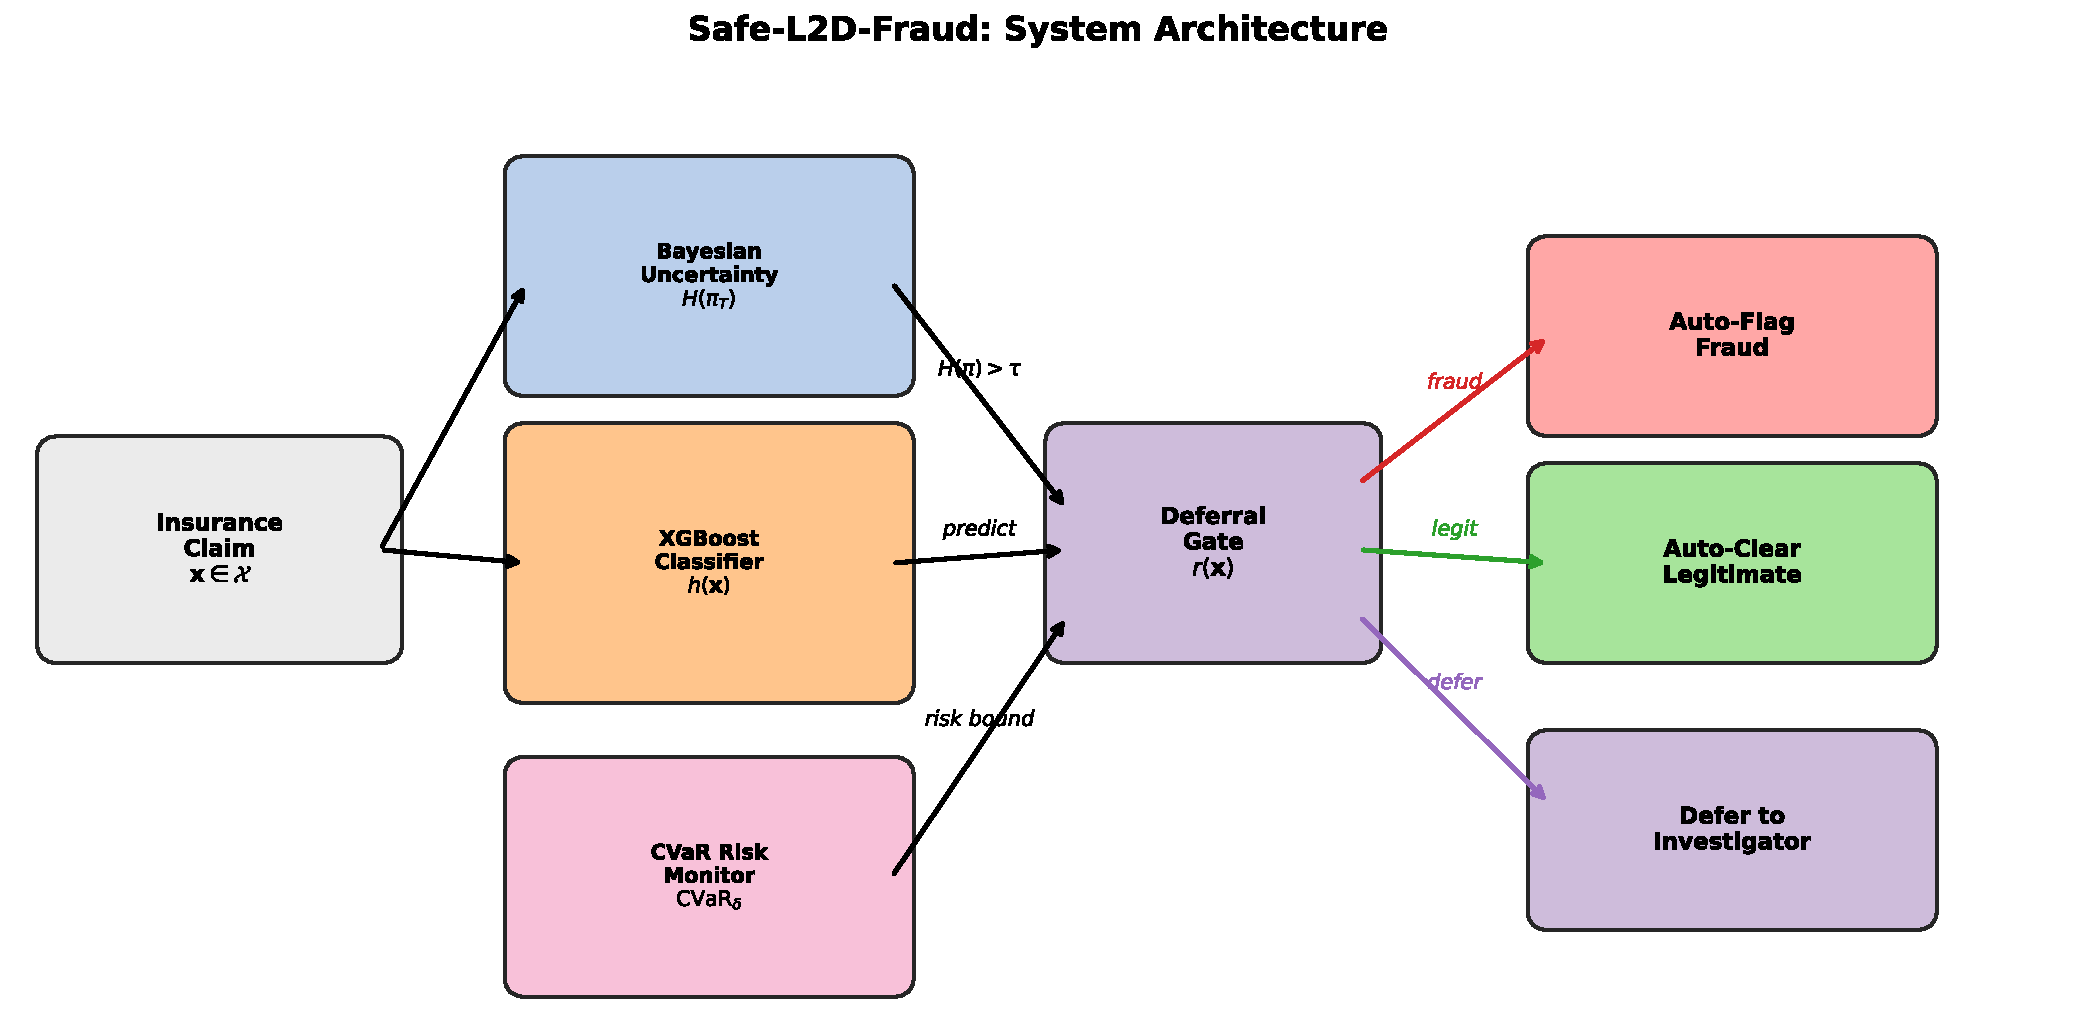
\includegraphics[width=\columnwidth]{figures/l2d_system_diagram.pdf}
    \caption{Safe-L2D-Fraud architecture. Claims flow through a Bayesian uncertainty module and XGBoost classifier. A CVaR-guided deferral gate routes uncertain claims to a human investigator, controlling tail risk on retained predictions.}
    \label{fig:system}
\end{figure}

\subsection{Bayesian Uncertainty Quantification}
\label{sec:method_bayes}

For each claim $\xx$, we estimate class-conditional densities $\hat{p}(x_k | y{=}1)$ and $\hat{p}(x_k | y{=}0)$ using Gaussian KDE on the training set, restricting to features validated by the domain-informed DAG (\Cref{sec:method_causal}). The posterior fraud probability $\pi_F$ is obtained via the sequential update in \Cref{eq:bayes_update}.

The entropy-based deferral signal is:
\begin{equation}
\begin{aligned}
U_{\text{Bayes}}(\xx)
&= H(\pi_F) \\
&= -\pi_F \log_2 \pi_F - (1{-}\pi_F)\log_2(1{-}\pi_F)
\end{aligned}
\label{eq:entropy_defer}
\end{equation}
This is maximised at $\pi_F = 0.5$ (maximum ambiguity) and decreases as $\pi_F$ moves toward 0 or 1. Claims with $U_{\text{Bayes}}(\xx) > \tau$ are candidates for deferral. \Cref{fig:class_cond} shows substantial class-conditional overlap in claim amount and policy age---the ambiguous region where deferral is most valuable.

\begin{figure}[H]
    \centering
    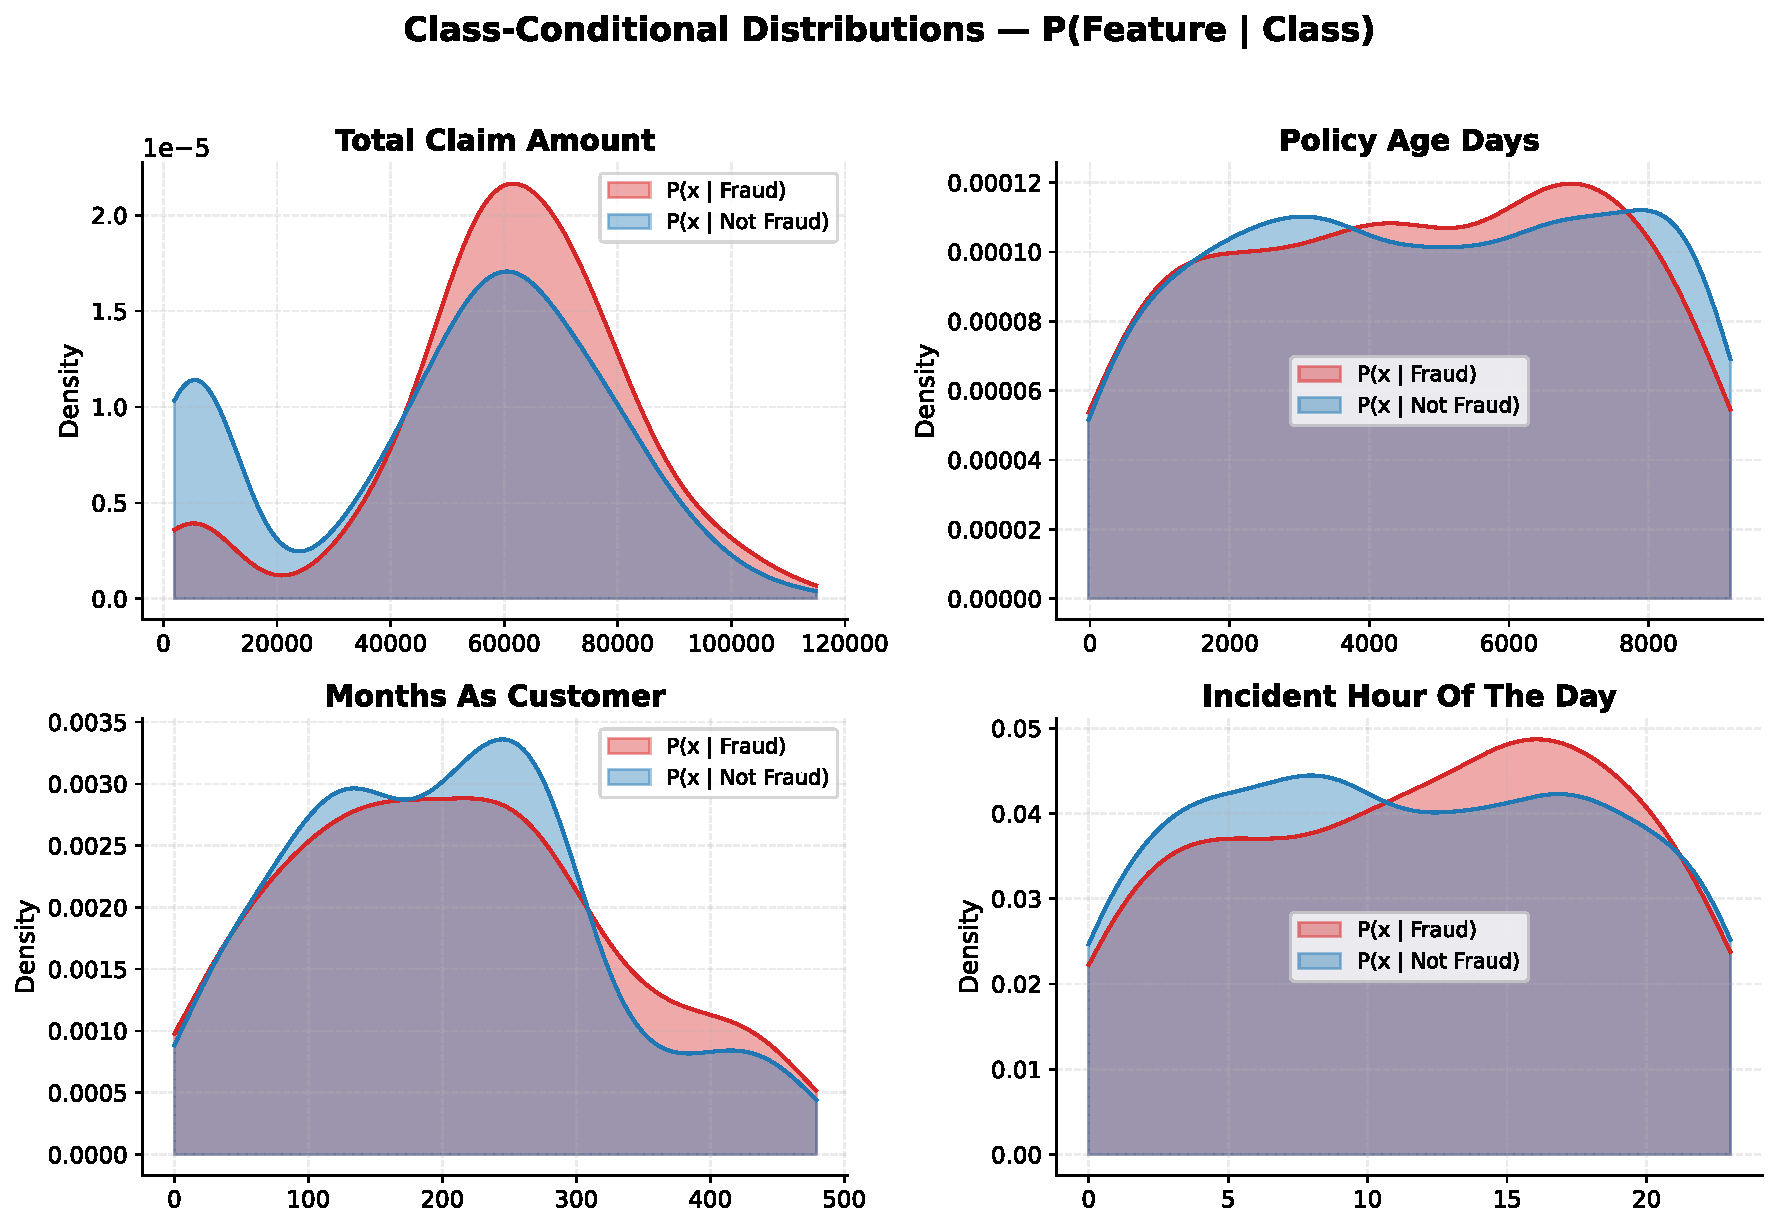
\includegraphics[width=\columnwidth]{figures/class_conditional_densities.pdf}
    \caption{Class-conditional densities $\hat{p}(x | y{=}1)$ vs $\hat{p}(x | y{=}0)$ for four features. Regions of high overlap correspond to high posterior entropy and trigger deferral.}
    \label{fig:class_cond}
\end{figure}

\subsection{Combined Deferral Rule}
\label{sec:method_cvar}

We combine the Bayesian entropy signal with the classifier's calibrated confidence to capture complementary sources of uncertainty:
\begin{equation}
    r(\xx) = \mathbf{1}\bigl[H(\pi_F) > \tau\bigr] \;\lor\; \mathbf{1}\bigl[\max_j \sigma_j(g(\xx)) < \kappa\bigr],
    \label{eq:combined_defer}
\end{equation}
where $\sigma_j(g(\xx))$ denotes the calibrated probability of class $j$ and $\kappa$ is a confidence threshold. The Bayesian posterior captures class-conditional overlap (generative uncertainty), while classifier confidence reflects decision-boundary separation (discriminative uncertainty). The OR combination is a simple design choice; learned fusion rules are left to future work.

The CVaR-penalised deferral threshold $\tau^*$ is selected by the objective in \Cref{eq:cvar_l2d}, sweeping $\tau$ over a grid while holding $\kappa$ fixed at 0.65 (chosen via preliminary validation; joint optimisation of $\tau$ and $\kappa$ is left to future work). The empirical CVaR on retained predictions is:
\begin{equation}
    \widehat{\cvar}_\delta = \frac{1}{\lceil \delta \cdot N_r \rceil} \sum_{i=1}^{\lceil \delta \cdot N_r \rceil} \ell_{(i)},
\end{equation}
where $\ell_{(1)} \geq \ell_{(2)} \geq \cdots$ are the sorted 0-1 losses of the $N_r$ non-deferred samples. The complete training procedure is given in Appendix~\ref{app:algorithm} (Section~D).

\subsection{Domain-Informed Feature Selection}
\label{sec:method_causal}

Using all features for Bayesian uncertainty risks deferring on spurious correlations that shift post-deployment. We build a domain-informed DAG (\Cref{fig:dag}) representing expected causal relationships between features and fraud \citep{pearl2009causality}, then retain only features with both a direct path to $y$ in the DAG \textit{and} positive KL divergence:
\begin{equation}
    D_{\text{KL}}^{(k)} = \int \hat{p}(x_k | y{=}1) \log \frac{\hat{p}(x_k | y{=}1)}{\hat{p}(x_k | y{=}0)} \, dx_k.
    \label{eq:kl_feature}
\end{equation}
This dual criterion selects features that are both structurally plausible and empirically discriminative. We do not claim to identify true causal parents; the DAG is an interpretable prior, and its advantage over standard feature selection (e.g., mutual information) has not been tested in controlled comparison.

\begin{figure}[H]
    \centering
    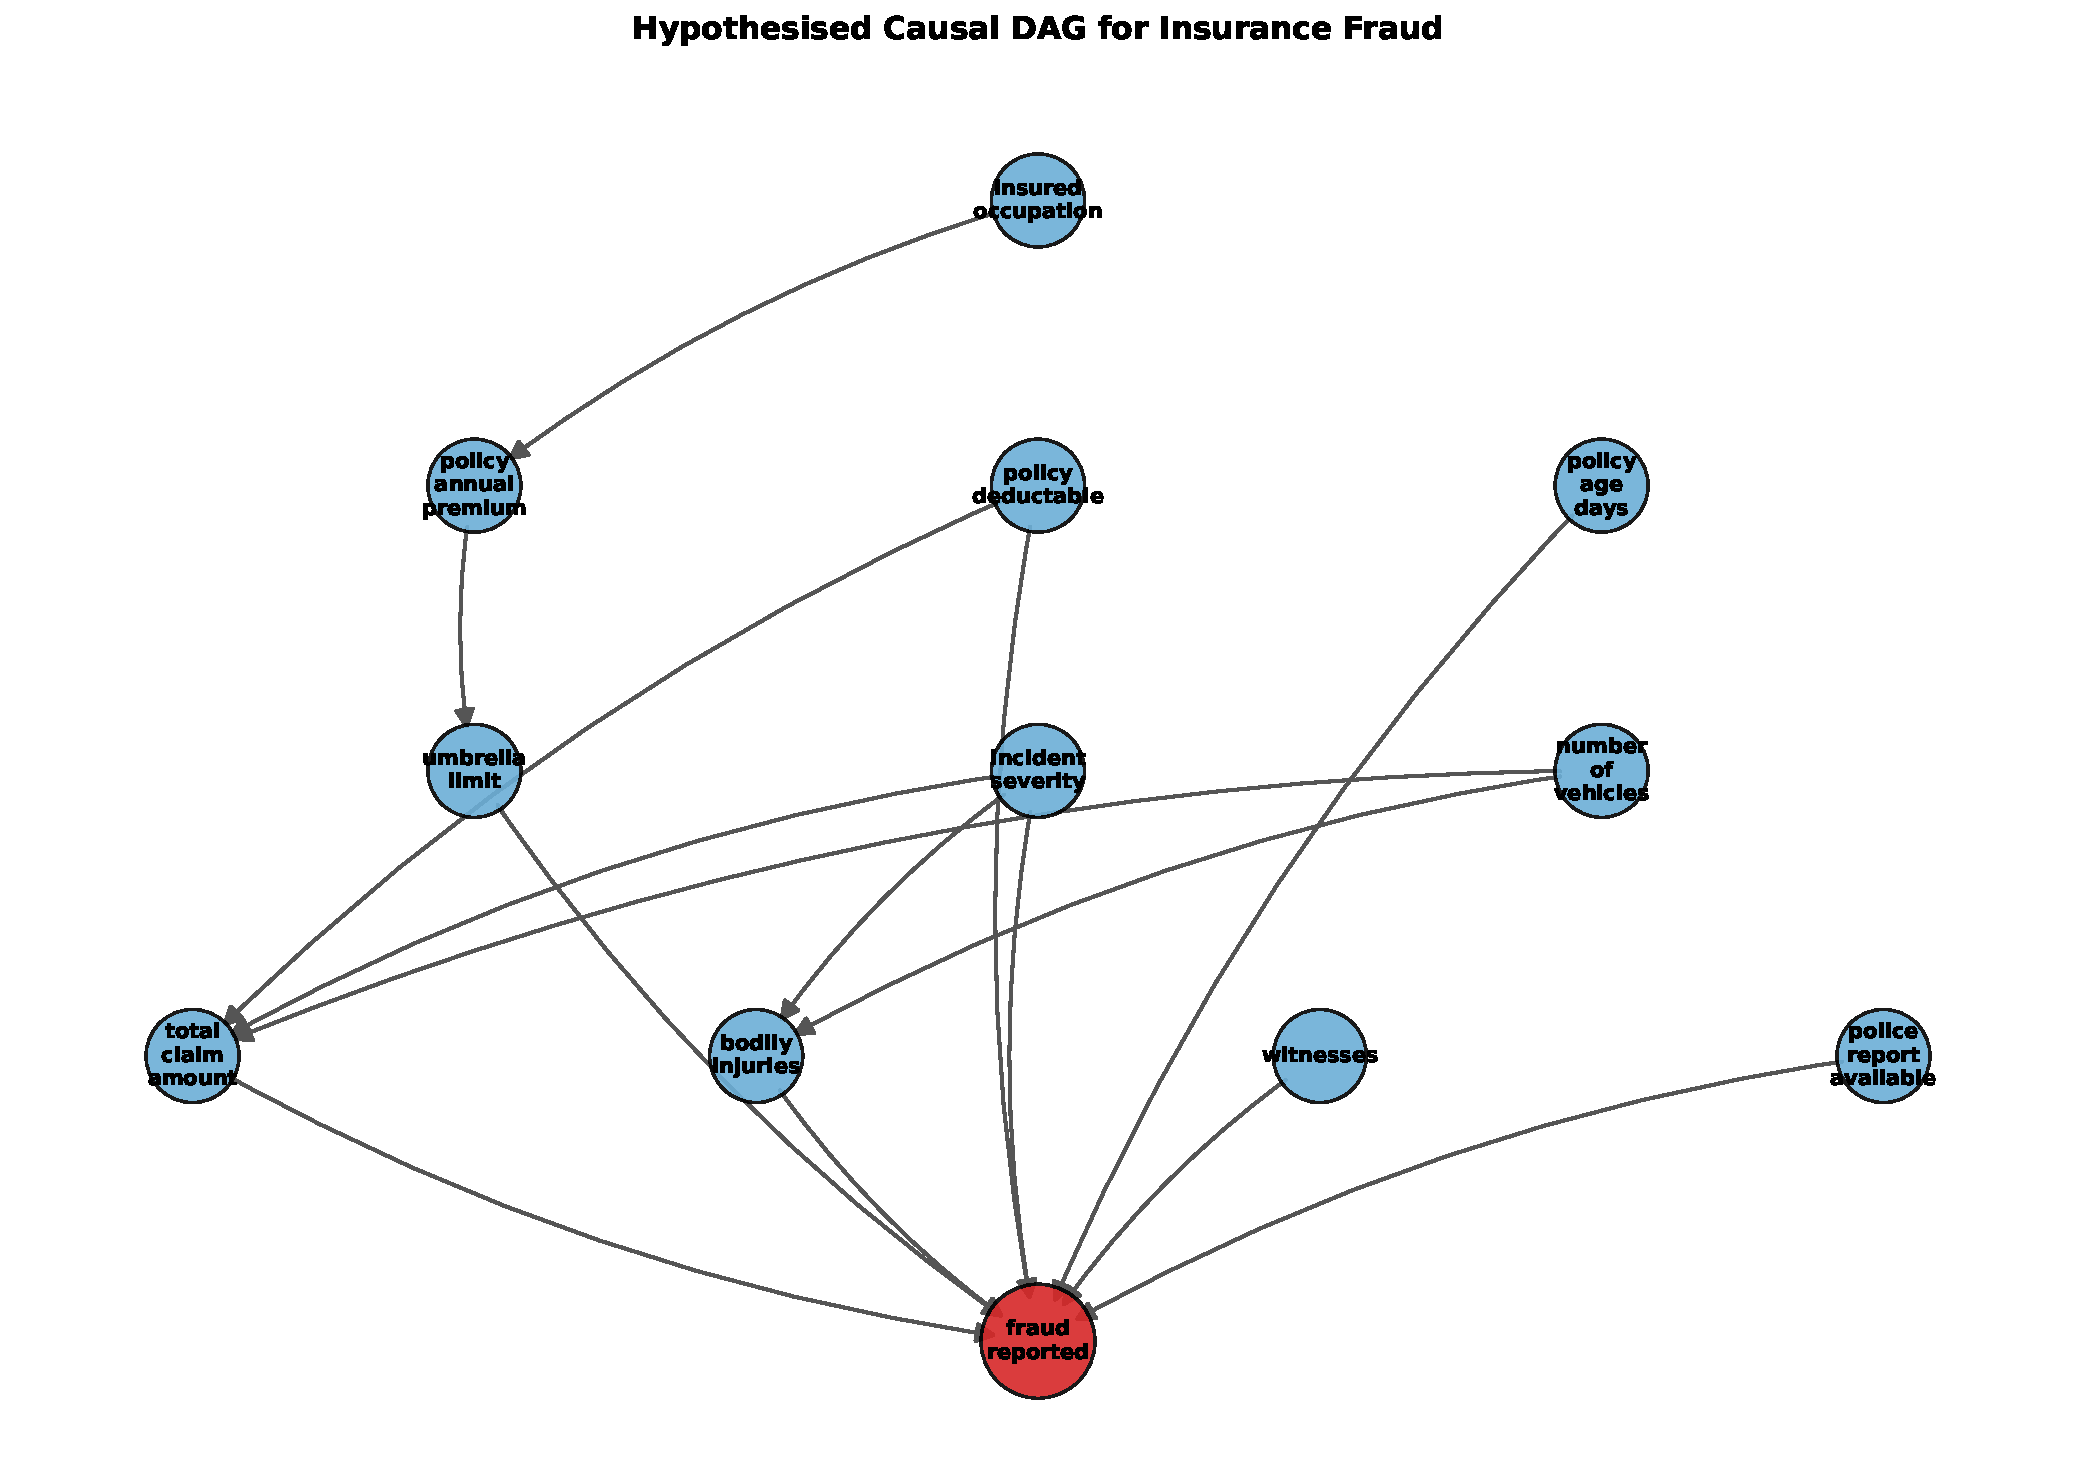
\includegraphics[width=\columnwidth]{figures/causal_dag.pdf}
    \caption{Domain-informed DAG for insurance fraud. Only variables with direct edges to \texttt{fraud\_reported} are used for Bayesian updating, reducing sensitivity to spurious correlations. The DAG is hypothesised from domain knowledge, not learned from data.}
    \label{fig:dag}
\end{figure}

\subsection{Off-Policy Evaluation}
\label{sec:method_ope}

To assess how Safe-L2D-Fraud would have performed on historical claims without deployment, we use off-policy evaluation (OPE) with three complementary estimators \citep{dudik2011doubly}: Direct Method (DM), Self-Normalised Importance Sampling (SNIPS, clipped at $w_{\max}{=}10$), and Doubly Robust (DR). Definitions are standard and given in \Cref{app:math}.

\noindent\textbf{Simulated behaviour policy.} Since historical investigator decisions are unavailable, we simulate $\pi_b$ via logistic regression on the training data. This introduces circularity ($\hat{r}$ and $\pi_b$ both learned from the same data), so our OPE results are a \textit{methodological illustration}, not counterfactual evidence. Real deployment would require actual adjudication records.
